\documentclass[tikz,border=8pt]{standalone}
\usepackage{amsmath,amssymb}
\usetikzlibrary{arrows.meta,calc,patterns}

\begin{document}
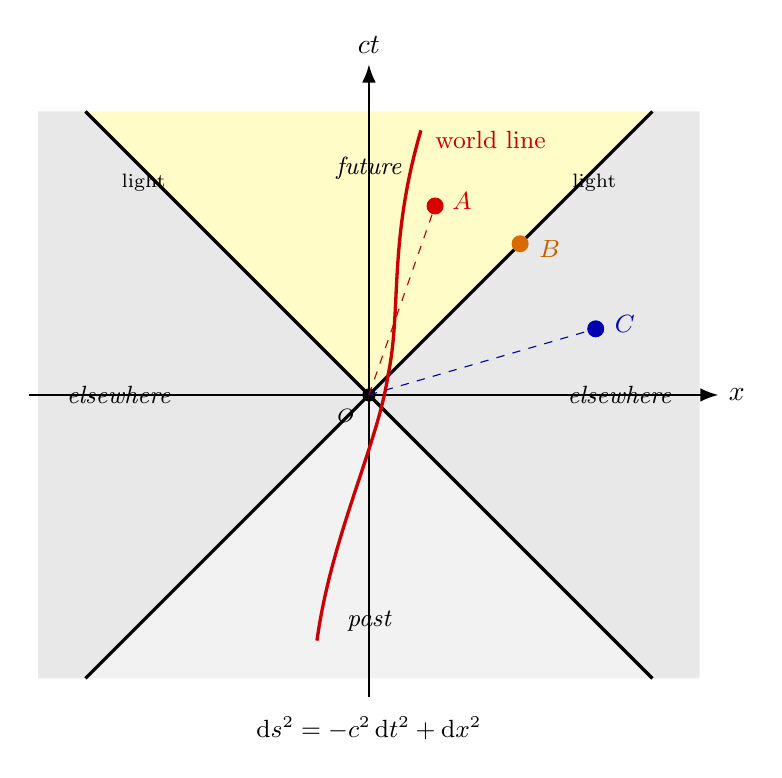
\begin{tikzpicture}[>=Latex, scale=1.2]

  % --- Background regions ---
  % Future light cone (light yellow shading)
  \fill[yellow!22] (0,0) -- (3.0, 3.0) -- (-3.0, 3.0) -- cycle;
  % Past light cone (very light gray)
  \fill[gray!10] (0,0) -- (3.0, -3.0) -- (-3.0, -3.0) -- cycle;
  % Spacelike regions (light gray)
  \fill[gray!18] (0,0) -- (3.0, 3.0) -- (3.5, 3.0) -- (3.5, -3.0) -- (3.0, -3.0) -- cycle;
  \fill[gray!18] (0,0) -- (-3.0, 3.0) -- (-3.5, 3.0) -- (-3.5, -3.0) -- (-3.0, -3.0) -- cycle;

  % --- Axes ---
  \draw[->, thick] (-3.6, 0) -- (3.7, 0) node[anchor=west] {$x$};
  \draw[->, thick] (0, -3.2) -- (0, 3.5) node[anchor=south] {$ct$};

  % --- Light cone (45 deg lines) ---
  \draw[very thick, black] (-3.0, -3.0) -- (3.0, 3.0);
  \draw[very thick, black] (3.0, -3.0) -- (-3.0, 3.0);

  % --- Region labels ---
  \node[font=\small\itshape, anchor=center] at (0, 2.4) {future};
  \node[font=\small\itshape, anchor=center] at (0, -2.4) {past};
  \node[font=\small\itshape, anchor=center] at (2.65, 0) {elsewhere};
  \node[font=\small\itshape, anchor=center] at (-2.65, 0) {elsewhere};

  % --- World line of an observer (red, timelike, slightly curved, stays inside cone) ---
  \draw[very thick, red!80!black, smooth]
    (-0.55, -2.6) .. controls (-0.40, -1.5) and (0.10, -0.5) ..
    (0.20, 0.2) .. controls (0.35, 0.9) and (0.20, 1.6) ..
    (0.55, 2.8);
  \node[red!80!black, font=\small, anchor=west] at (0.6, 2.7) {world line};

  % --- Origin event ---
  \fill[black] (0,0) circle (0.07);
  \node[font=\scriptsize, anchor=north east] at (-0.05, -0.05) {$O$};

  % --- Event A: timelike future (inside future cone) ---
  \fill[red!85!black] (0.7, 2.0) circle (0.09);
  \node[font=\small, red!85!black, anchor=west] at (0.78, 2.05) {$A$};
  % dashed line from O to A
  \draw[dashed, red!75!black] (0,0) -- (0.7, 2.0);

  % --- Event B: lightlike (on the cone) ---
  \fill[orange!85!black] (1.6, 1.6) circle (0.09);
  \node[font=\small, orange!75!black, anchor=west] at (1.7, 1.55) {$B$};

  % --- Event C: spacelike (elsewhere) ---
  \fill[blue!70!black] (2.4, 0.7) circle (0.09);
  \node[font=\small, blue!70!black, anchor=west] at (2.5, 0.75) {$C$};
  \draw[dashed, blue!65!black] (0,0) -- (2.4, 0.7);

  % --- ds^2 formula at the bottom ---
  \node[font=\small, anchor=north] at (0, -3.3)
    {$\mathrm ds^2 = -c^2\,\mathrm dt^2 + \mathrm dx^2$};

  % --- A small label hinting which line is the light cone ---
  \node[font=\scriptsize, anchor=south west] at (2.05, 2.05) {light};
  \node[font=\scriptsize, anchor=south east] at (-2.05, 2.05) {light};

\end{tikzpicture}
\end{document}
